\chapter{Analisi dei requisiti}
\label{cap:analisi-requisiti}

\intro{Breve introduzione al capitolo}\\

\section{Casi d'uso}

Per lo studio dei casi di utilizzo del prodotto sono stati creati dei diagrammi.
I diagrammi dei casi d'uso (in inglese \emph{Use Case Diagram}) sono diagrammi di tipo \gls{uml} dedicati alla descrizione delle funzioni o servizi offerti da un sistema, così come sono percepiti e utilizzati dagli attori che interagiscono col sistema stesso.
Di seguito i casi d'uso di interesse e le loro descrizioni testuali accompagnate dalle condizioni necessarie per accedere alle relative funzionalità offerte dal sistema sviluppato. 
I diagrammi sono stati raggruppati per funzionalità accessibili da ciascuna finestra dell'applicazione 

\begin{figure}[!h] 
    \centering 
    \makebox[\textwidth]{
    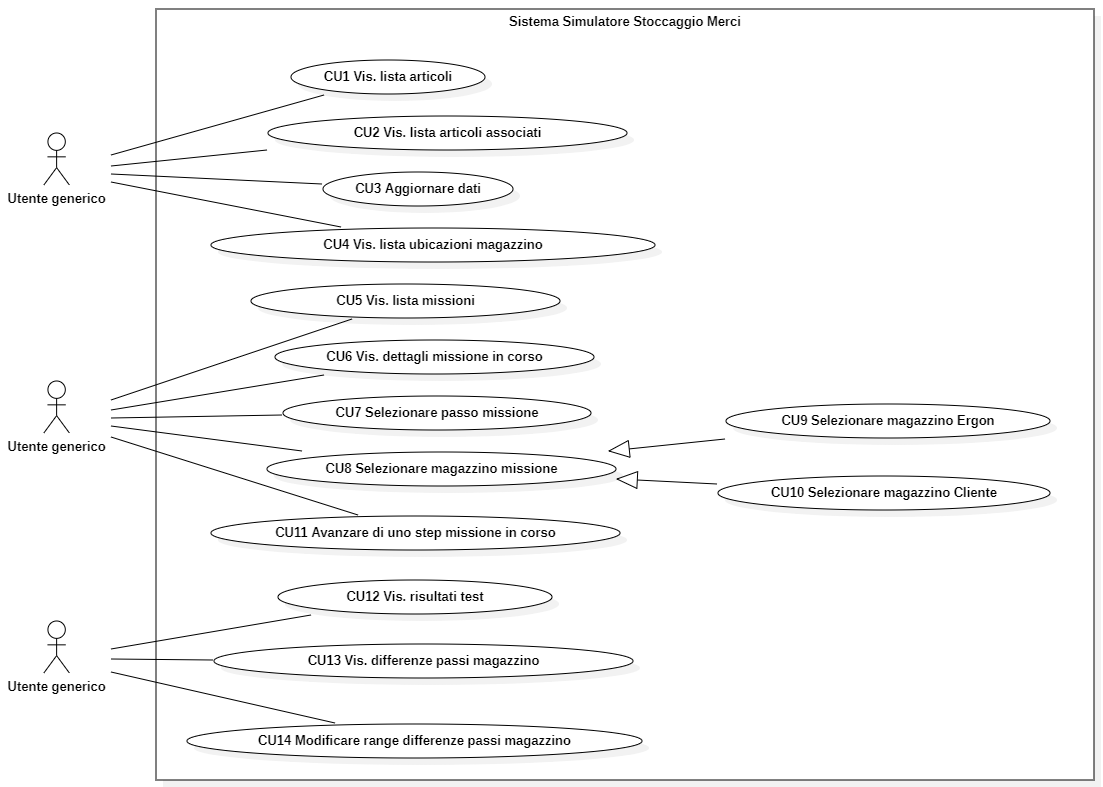
\includegraphics[width=1.5\columnwidth]{../images/usecase/generale} 
    }
    \caption{Casi d'uso - Sky level}
\end{figure}


\begin{usecase}{1}{Vis. lista articoli}
\usecaseactors{Utente generico}
\usecasepre{Nessuna}
\usecasedesc{La finestra mette a disposizione la visualizzazione della lista degli articoli con unità di misura "FS" che sono presenti in almeno un ordine cliente}
\usecasepost{L'utente visualizza la lista degli articoli con unità di misura "FS" che sono presenti in almeno un ordine cliente}
\textbf{\\Scenario Principale:}
\begin{itemize}
    \item L'utente apre la finestra per visualizzare la lista degli articoli.
\end{itemize}
\label{uc:scenario-principale}
\end{usecase}
%%%%%%%%%%%%%%%%%%%%%%%%%%%%%%%%%%%%%%%%%%%%%%%%%%%%%%
\begin{usecase}{2}{Vis. lista articoli associati}
    \usecaseactors{Utente generico}
    \usecasepre{Nessuna}
\usecasedesc{La finestra mette a disposizione la visualizzazione della lista degli articoli associati all'articolo selezionato nella lista articoli}
\usecasepost{L'utente visualizza la lista degli articoli associati all'articolo selezionato}
\textbf{\\Scenario Principale:}
\begin{itemize}
    \item L'utente apre la finestra per visualizzare la lista degli articoli;
    \item L'utente seleziona dalla lista articoli l'articolo di cui vuole visualizzare gli articoli associati.
\end{itemize}
\label{uc:scenario-principale}
\end{usecase}
%%%%%%%%%%%%%%%%%%%%%%%%%%%%%%%%%%%%%%%%%%%%%%%%%%%%%%
\begin{usecase}{3}{Aggiornare dati}
\usecaseactors{Utente generico}
\usecasepre{L'utente dispone delle autorizzazioni necessarie a interagire con il database}
\usecasedesc{L'utente aggiorna i dati relativi alla frequenza di vendita degli articoli e alla frequenza di associazione tra articoli presenti a database}
\textbf{\\Postcondizioni:}
\begin{itemize}
    \item I dati sulla frequenza di vendita e le associazioni degli articoli sono aggiornati a database.
\end{itemize}
\textbf{\\Scenario Principale:}
\begin{itemize}
    \item L'utente utilizza il comando "Aggiorna dati" per aggiornare i dati relativi alla frequenza di vendita e associazioni tra articoli presenti a database.
\end{itemize}
\label{uc:scenario-principale}
\end{usecase}
%%%%%%%%%%%%%%%%%%%%%%%%%%%%%%%%%%%%%%%%%%%%%%%%%%%%%%
\begin{usecase}{4}{Vis. lista ubicazioni magazzino}
\usecaseactors{Utente generico}
\usecasepre{L'utente ha avviato una simulazione di prelievo}
\usecasedesc{L'utente visualizza la disposizione degli articoli a magazzino}
\textbf{\\Postcondizioni:}
\begin{itemize}
    \item La disposizione degli articoli a magazzino è visibile.
\end{itemize}
\textbf{\\Scenario Principale:}
\begin{itemize}
    \item L'utente utilizza il comando "Avvia simulazione" per avviare una simulazione di prelievo.
\end{itemize}
\label{uc:scenario-principale}
\end{usecase}
%%%%%%%%%%%%%%%%%%%%%%%%%%%%%%%%%%%%%%%%%%%%%%%%%%%%%%
\begin{usecase}{5}{Vis. lista missioni}
\usecaseactors{Utente generico}
\usecasepre{L'utente ha avviato una simulazione di prelievo}
\usecasedesc{L'utente visualizza la missione di prelievo in corso e passate relative alla simulazione di prelievo}
\textbf{\\Postcondizioni:}
\begin{itemize}
    \item La missione di prelievo in corso è visibile;
    \item Le missioni di prelievo passate sono visibili.
\end{itemize}
\textbf{\\Scenario Principale:}
\begin{itemize}
    \item L'utente utilizza il comando "Avvia simulazione" per avviare una simulazione di prelievo.
\end{itemize}
\label{uc:scenario-principale}
\end{usecase}
%%%%%%%%%%%%%%%%%%%%%%%%%%%%%%%%%%%%%%%%%%%%%%%%%%%%%%
\begin{usecase}{6}{Vis. dettagli missione in corso}
\usecaseactors{Utente generico}
\usecasepre{L'utente ha avviato una simulazione di prelievo}
\usecasedesc{L'utente visualizza lo stato della missione in corso}
\textbf{\\Postcondizioni:}
\begin{itemize}
    \item Lo stato della missione in corso è visibile.
\end{itemize}
\textbf{\\Scenario Principale:}
\begin{itemize}
    \item L'utente utilizza il comando "Avvia simulazione" per avviare una simulazione di prelievo.
\end{itemize}
\label{uc:scenario-principale}
\end{usecase}
%%%%%%%%%%%%%%%%%%%%%%%%%%%%%%%%%%%%%%%%%%%%%%%%%%%%%%
\begin{usecase}{7}{Selezionare passo missione}
\usecaseactors{Utente generico}
\usecasepre{L'utente ha avviato una simulazione di prelievo}
\usecasedesc{L'utente modifica il passo associazioni con cui vengono disposti gli articoli a magazzino}
\textbf{\\Postcondizioni:}
\begin{itemize}
    \item La simulazione di prelievo è ripristinata allo stato iniziale;
    \item La disposizione degli articoli a magazzino è aggiornata secondo il passo selezionato dall'utente.
\end{itemize}
\textbf{\\Scenario Principale:}
\begin{itemize}
    \item L'utente modifica il passo missione utilizzando la form dedicata.
\end{itemize}
\label{uc:scenario-principale}
\end{usecase}
%%%%%%%%%%%%%%%%%%%%%%%%%%%%%%%%%%%%%%%%%%%%%%%%%%%%%%
\begin{usecase}{8}{Selezionare magazzino missione}
    \textbf{\\Generalizzazione di:}
\begin{itemize}
    \item CU9 Selezionare magazzino Ergon;
    \item CU10 Selezionare magazzino cliente.
\end{itemize}
\usecaseactors{Utente generico}
\usecasepre{L'utente ha avviato una simulazione di prelievo}
\usecasedesc{L'utente seleziona il magazzino sul quale effettuare la simulazione}
\textbf{\\Postcondizioni:}
\begin{itemize}
    \item La simulazione di prelievo è ripristinata allo stato iniziale;
    \item La disposizione degli articoli a magazzino è aggiornata secondo il magazzino selezionato dall'utente.
\end{itemize}
\textbf{\\Scenario Principale:}
\begin{itemize}
    \item L'utente seleziona il magazzino sul quale effettuare la missione utilizzando la form dedicata.
\end{itemize}
\label{uc:scenario-principale}
\end{usecase}
%%%%%%%%%%%%%%%%%%%%%%%%%%%%%%%%%%%%%%%%%%%%%%%%%%%%%%
\begin{usecase}{9}{Selezionare magazzino Ergon}
\usecaseactors{Utente generico}
\usecasepre{L'utente ha avviato una simulazione di prelievo}
\usecasedesc{L'utente seleziona il magazzino Ergon sul quale effettuare la simulazione. Il magazzino Ergon è caratterizzato da una disposizione degli articoli che segue il passo associazione
articoli selezionato dall'utente}
\textbf{\\Postcondizioni:}
\begin{itemize}
    \item La simulazione di prelievo è ripristinata allo stato iniziale;
    \item La disposizione degli articoli a magazzino è aggiornata secondo il magazzino Ergon rispettando il passo selezionato dall'utente;
    \item La funzionalità di selezione passo magazzino è abilitata.
\end{itemize}
\textbf{\\Scenario Principale:}
\begin{itemize}
    \item L'utente seleziona il magazzino Ergon sul quale effettuare la missione utilizzando la form dedicata.
\end{itemize}
\label{uc:scenario-principale}
\end{usecase}
%%%%%%%%%%%%%%%%%%%%%%%%%%%%%%%%%%%%%%%%%%%%%%%%%%%%%%
\begin{usecase}{10}{Selezionare magazzino cliente}
\usecaseactors{Utente generico}
\usecasepre{L'utente ha avviato una simulazione di prelievo}
\usecasedesc{L'utente seleziona il magazzino cliente sul quale effettuare la simulazione. Il magazzino cliente rispetta fedelmente la disposizione attuale del magazzino cliente e non applica un passo 
associazione prodotti}
\textbf{\\Postcondizioni:}
\begin{itemize}
    \item La simulazione di prelievo è ripristinata allo stato iniziale;
    \item La disposizione degli articoli a magazzino è aggiornata secondo il magazzino cliente;
    \item La funzionalità di selezione passo magazzino è disabilitata.
\end{itemize}
\textbf{\\Scenario Principale:}
\begin{itemize}
    \item L'utente seleziona il magazzino cliente sul quale effettuare la missione utilizzando la form dedicata.
\end{itemize}
\label{uc:scenario-principale}
\end{usecase}
%%%%%%%%%%%%%%%%%%%%%%%%%%%%%%%%%%%%%%%%%%%%%%%%%%%%%%
\begin{usecase}{11}{Avanzare di uno step missione in corso}
\usecaseactors{Utente generico}
\textbf{\\Precondizioni:}
\begin{itemize}
    \item Nella simulazionie di prelievo è presente almeno una missione non terminata;
    \item La missione attuale si trova ad uno step di partenza.
\end{itemize}
\usecasedesc{L'utente avanza di uno step nella missione in corso. Avanzare di uno step permette di visualizzare lo stato del carrello alla fermata successiva rispetto allo step missione attuale}
\textbf{\\Postcondizioni:}
\begin{itemize}
    \item La missione attuale si trova allo step successivo allo step di partenza.
\end{itemize}
\textbf{\\Scenario Principale:}
\begin{itemize}
    \item L'utente utilizza il comando "Avanza step missione" per avanzare di uno step missione.
\end{itemize}
\label{uc:scenario-principale}
\end{usecase}
%%%%%%%%%%%%%%%%%%%%%%%%%%%%%%%%%%%%%%%%%%%%%%%%%%%%%%
\begin{usecase}{12}{Vis. risultati test}
\usecaseactors{Utente generico}
\usecasepre{Nessuna}
\usecasedesc{L'utente visualizza i risultati della simulazione effettuata sul magazzino cliente e di tutte le simulazioni effettuate sul magazzino Ergon a tutti i passi previsti dal sistema di 
simulazione}
\usecasepost{I risultati di tutte le simulazioni effettuate sono visibili all'utente}
\textbf{\\Scenario Principale:}
\begin{itemize}
    \item L'utente utilizza il comando "Visualizza risultati test" per visualizzare i risultati dei test.
\end{itemize}
\label{uc:scenario-principale}
\end{usecase}
%%%%%%%%%%%%%%%%%%%%%%%%%%%%%%%%%%%%%%%%%%%%%%%%%%%%%%
\begin{usecase}{13}{Vis. differenze passi magazzino}
\usecaseactors{Utente generico}
\usecasepre{Nessuna}
\usecasedesc{L'utente visualizza le differenze tra le diverse configurazioni di magazzino Ergon che dipendono dai passi associazioni.Le differenze vengono visualizzate tenendo conto 
del range di ubicazioni selezionate dell'utente entro il quale si vogliono visualizzare le differenze tra le configurazioni di magazzino}
\usecasepost{Le differenze tra le diverse configurazioni di magazzino Ergon sono visibili all'utente}
\textbf{\\Scenario Principale:}
\begin{itemize}
    \item L'utente utilizza il comando "Visualizza differenze passi" per visualizzare le differenze tra le diverse configurazioni di magazzino Ergon.
\end{itemize}
\label{uc:scenario-principale}
\end{usecase}
%%%%%%%%%%%%%%%%%%%%%%%%%%%%%%%%%%%%%%%%%%%%%%%%%%%%%%
\begin{usecase}{14}{Modificare range differenze passi magazzino}
\usecaseactors{Utente generico}
\usecasepre{L'utente visualizza le differenze passi magazzino in un range di partenza}
\usecasedesc{L'utente modifica il range differenze passi magazzino per visualizzare le differenze tra le diverse configurazioni di magazzino in un range diverso da quello di partenza}
\textbf{\\Postcondizioni:}
\begin{itemize}
    \item Il range di visualizzazione differenze passi magazzino è stato modificato;
    \item Le differenze tra le configurazioni di magazzino sono state aggiornate secondo il range impostato;
    \item Le differenze tra le diverse configurazioni di magazzino Ergon sono visibili all'utente.
\end{itemize}
\textbf{\\Scenario Principale:}
\begin{itemize}
    \item L'utente utilizza il comando "Modifica range" per aggiornare la visualizzazione delle differenze tra le diverse configurazioni di magazzino Ergon.
\end{itemize}
\label{uc:scenario-principale}
\end{usecase} 
%%%%%%%%%%%%%%%%%%%%%%%%%%%%%%%%%%%%%%%%%%%%%%%%%%%%%%
\begin{figure}[!h] 
    \centering 
    \makebox[\textwidth]{
    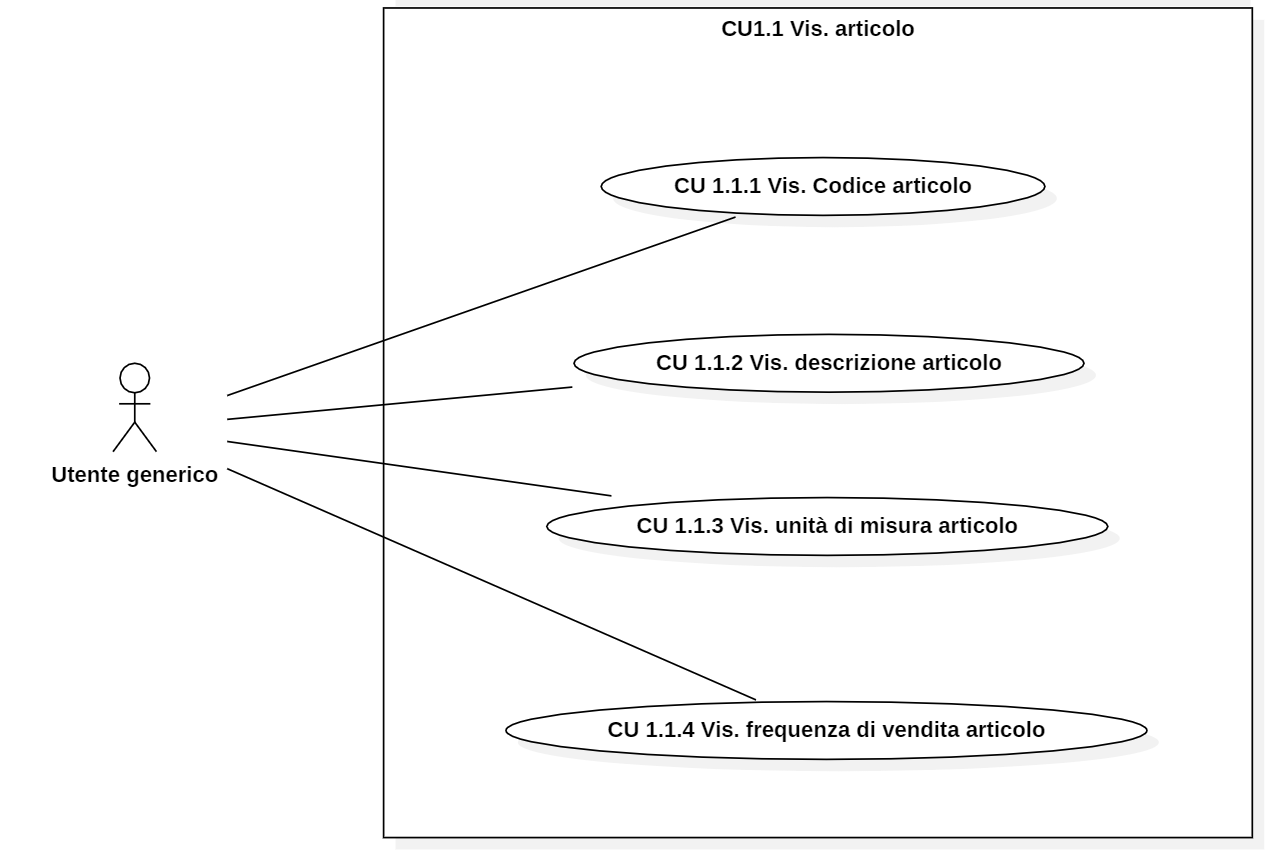
\includegraphics[width=1.2\columnwidth]{../images/usecase/form1/CU1_1} 
    }
    \caption{Casi d'uso - CU1.1 Vis. articolo}
\end{figure}

\begin{usecase}{1.1}{Vis. articolo}
    \usecaseactors{Utente generico}
    \usecasepre{Nessuna}
    \usecasedesc{L'utente visualizza un articolo presente nella lista articoli}
    \usecasepost{L'articolo è visibile all'utente}
    \label{uc:scenario-principale}
\end{usecase}
%%%%%%%%%%%%%%%%%%%%%%%%%%%%%%%%%%%%%%%%%%%%%%%%%%%%%%
\begin{usecase}{1.1.1}{Vis. Codice articolo}
    \usecaseactors{Utente generico}
    \usecasepre{Nessuna}
    \usecasedesc{L'utente visualizza il codice articolo dell'articolo presente nella lista articoli. Il codice articolo è un identificatore univoco per un articolo}
    \usecasepost{Il codice dell'articolo è visibile all'utente}
    \label{uc:scenario-principale}
\end{usecase}
%%%%%%%%%%%%%%%%%%%%%%%%%%%%%%%%%%%%%%%%%%%%%%%%%%%%%%
\begin{usecase}{1.1.2}{Vis. descrizione articolo}
    \usecaseactors{Utente generico}
    \usecasepre{Nessuna}
    \usecasedesc{L'utente visualizza la descrizione dell'articolo presente nella lista articoli}
    \usecasepost{La descrizione dell'articolo è visibile all'utente}
    \label{uc:scenario-principale}
\end{usecase}
%%%%%%%%%%%%%%%%%%%%%%%%%%%%%%%%%%%%%%%%%%%%%%%%%%%%%%
\begin{usecase}{1.1.3}{Vis. unità di misura articolo}
    \usecaseactors{Utente generico}
    \usecasepre{Nessuna}
    \usecasedesc{L'utente visualizza l'unità di misura dell'articolo presente nella lista articoli}
    \usecasepost{L'unità di misura dell'articolo è visibile all'utente}
    \label{uc:scenario-principale}
\end{usecase}
%%%%%%%%%%%%%%%%%%%%%%%%%%%%%%%%%%%%%%%%%%%%%%%%%%%%%%
\begin{usecase}{1.1.4}{Vis. frequenza di vendita articolo}
    \usecaseactors{Utente generico}
    \usecasepre{Nessuna}
    \usecasedesc{L'utente visualizza la frequenza di vendita dell'articolo presente nella lista articoli.La frequenza di vendita di un articolo corrisponde al numero di volte che 
    l'articolo compare all'interno degli ordini cliente}
    \usecasepost{La frequenza di vendita dell'articolo è visibile all'utente}
    \label{uc:scenario-principale}
\end{usecase}
%%%%%%%%%%%%%%%%%%%%%%%%%%%%%%%%%%%%%%%%%%%%%%%%%%%%%%
\begin{figure}[!h] 
    \centering 
    \makebox[\textwidth]{
    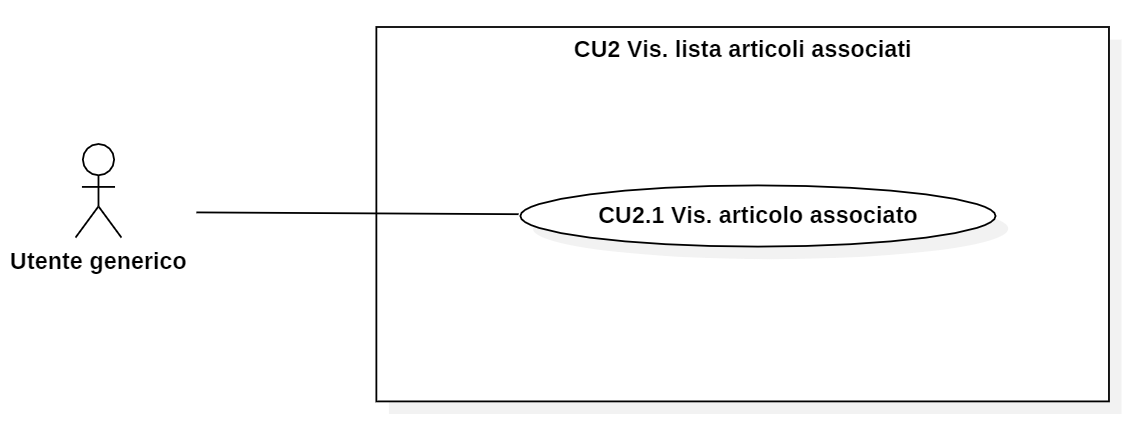
\includegraphics[width=1.2\columnwidth]{../images/usecase/form1/CU2} 
    }
    \caption{Casi d'uso - CU2 Vis. lista articoli associati}
\end{figure}

\begin{usecase}{2}{Vis. lista articoli associati}
    \usecaseactors{Utente generico}
    \usecasepre{Nessuna}
    \usecasedesc{L'utente visualizza la lista degli articoli associati. Gli articoli associati ad un articolo sono gli articoli che compaiono negli stessi ordini dell'articolo che si sta considerando}
    \usecasepost{La lista degli articoli associati è visibile all'utente}
    \label{uc:scenario-principale}
\end{usecase}
%%%%%%%%%%%%%%%%%%%%%%%%%%%%%%%%%%%%%%%%%%%%%%%%%%%%%%
\begin{figure}[!h] 
    \centering 
    \makebox[\textwidth]{
    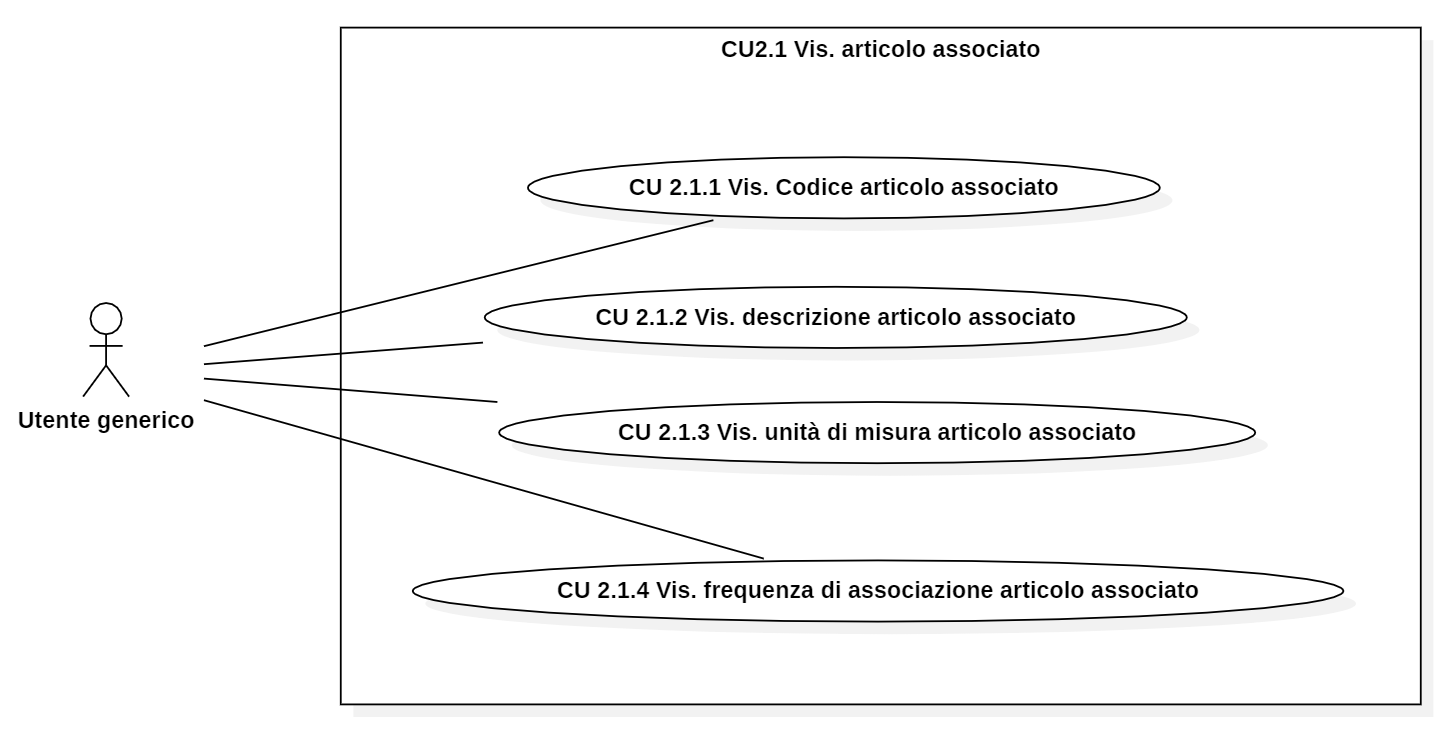
\includegraphics[width=1.3\columnwidth]{../images/usecase/form1/CU2_1} 
    }
    \caption{Casi d'uso - CU2.1 Vis. articolo associato}
\end{figure}

\begin{usecase}{2.1}{Vis. articolo associato}
    \usecaseactors{Utente generico}
    \usecasepre{Nessuna}
    \usecasedesc{L'utente visualizza un articolo presente nella lista articoli associati}
    \usecasepost{L'articolo associato è visibile all'utente}
    \label{uc:scenario-principale}
\end{usecase}
%%%%%%%%%%%%%%%%%%%%%%%%%%%%%%%%%%%%%%%%%%%%%%%%%%%%%%
\begin{usecase}{2.1.1}{Vis. Codice articolo associato}
    \usecaseactors{Utente generico}
    \usecasepre{Nessuna}
    \usecasedesc{L'utente visualizza il codice articolo dell'articolo associato presente nella lista articoli associati. Il codice articolo è un identificatore univoco per un articolo}
    \usecasepost{Il codice dell'articolo associato è visibile all'utente}
    \label{uc:scenario-principale}
\end{usecase}
%%%%%%%%%%%%%%%%%%%%%%%%%%%%%%%%%%%%%%%%%%%%%%%%%%%%%%
\begin{usecase}{2.1.1}{Vis. descrizione articolo associato}
    \usecaseactors{Utente generico}
    \usecasepre{Nessuna}
    \usecasedesc{L'utente visualizza la descrizione dell'articolo associato presente nella lista articoli associati}
    \usecasepost{la descrizione dell'articolo associato è visibile all'utente}
    \label{uc:scenario-principale}
\end{usecase}
%%%%%%%%%%%%%%%%%%%%%%%%%%%%%%%%%%%%%%%%%%%%%%%%%%%%%%
\begin{usecase}{2.1.1}{Vis. unità di misura articolo associato}
    \usecaseactors{Utente generico}
    \usecasepre{Nessuna}
    \usecasedesc{L'utente visualizza l'unità di misura dell'articolo associato presente nella lista articoli associati}
    \usecasepost{L'unità di misura dell'articolo associato è visibile all'utente}
    \label{uc:scenario-principale}
\end{usecase}
%%%%%%%%%%%%%%%%%%%%%%%%%%%%%%%%%%%%%%%%%%%%%%%%%%%%%%
\begin{usecase}{2.1.1}{Vis. frequenza di associazione articolo associato}
    \usecaseactors{Utente generico}
    \usecasepre{Nessuna}
    \usecasedesc{L'utente visualizza la frequenza di associazione dell'articolo associato presente nella lista articoli associati.La frequenza di associazione corrisponde al numero di volte in cui
    l'articolo associato compare all'interno degli ordini cliente con l'articolo selezionato dalla lista articoli}
    \usecasepost{La frequenza di associazione dell'articolo associato è visibile all'utente}
    \label{uc:scenario-principale}
\end{usecase}

%%%%%%%%%%%%%%%%%%%%%%%%%%%%%%%%%%%%%%%%%%%%%%%%%%%%%%
\begin{figure}[!h] 
    \centering 
    \makebox[\textwidth]{
    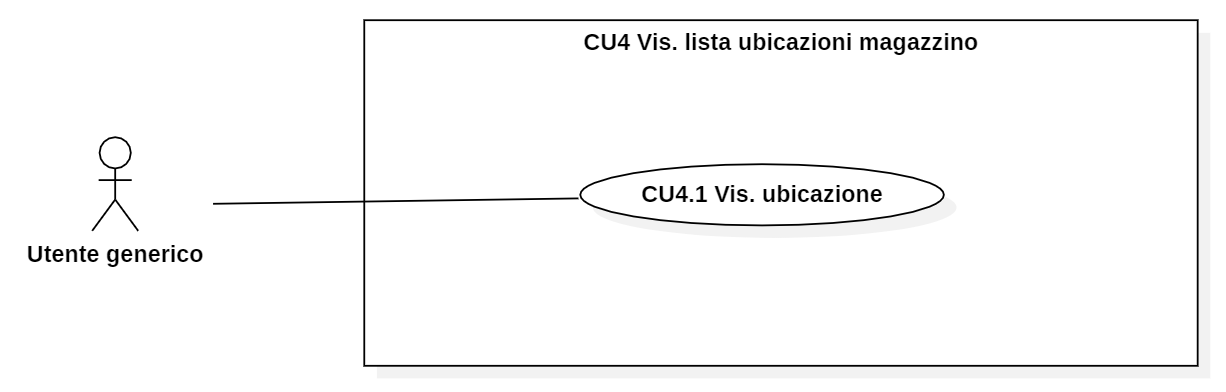
\includegraphics[width=1.2\columnwidth]{../images/usecase/form2/CU4} 
    }
    \caption{Casi d'uso - CU4 Vis. lista ubicazioni magazzino}
\end{figure}
%%%%%%%%%%%%%%%%%%%%%%%%%%%%%%%%%%%%%%%%%%%%%%%%%%%%%%
\begin{usecase}{4}{Vis. lista ubicazioni magazzino}
    \usecaseactors{Utente generico}
    \usecasepre{Nessuna}
    \usecasedesc{L'utente visualizza la lista delle ubicazioni del magazzino}
    \usecasepost{La lista delle ubicazioni del magazzino è visibile all'utente}
    \label{uc:scenario-principale}
\end{usecase}
%%%%%%%%%%%%%%%%%%%%%%%%%%%%%%%%%%%%%%%%%%%%%%%%%%%%%%
\begin{figure}[!h] 
    \centering 
    \makebox[\textwidth]{
    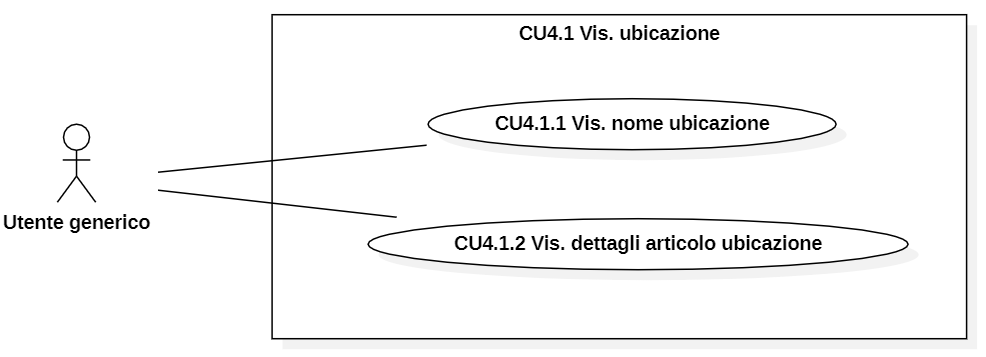
\includegraphics[width=1.2\columnwidth]{../images/usecase/form2/CU4_1} 
    }
    \caption{Casi d'uso - CU4.1 Vis. ubicazione}
\end{figure}
%%%%%%%%%%%%%%%%%%%%%%%%%%%%%%%%%%%%%%%%%%%%%%%%%%%%%%
\begin{usecase}{4.1}{Vis. ubicazione}
    \usecaseactors{Utente generico}
    \usecasepre{Nessuna}
    \usecasedesc{L'utente visualizza un'ubicazione di magazzino}
    \usecasepost{L'ubicazione del magazzino è visibile all'utente}
    \label{uc:scenario-principale}
\end{usecase}
%%%%%%%%%%%%%%%%%%%%%%%%%%%%%%%%%%%%%%%%%%%%%%%%%%%%%%
\begin{usecase}{4.1.1}{Vis. nome ubicazione}
    \usecaseactors{Utente generico}
    \usecasepre{Nessuna}
    \usecasedesc{L'utente visualizza il nome dell'ubicazione di magazzino. Il nome segue una numerazione incrementale che corrisponde alla posizione in cui si trova l'ubicazione
    nel magazzino. Minore è il numero dell'ubicazione prima verrà visitata dal carrello per il prelievo degli articoli}
    \usecasepost{Il nome dell'ubicazione è visibile all'utente}
    \label{uc:scenario-principale}
\end{usecase}
%%%%%%%%%%%%%%%%%%%%%%%%%%%%%%%%%%%%%%%%%%%%%%%%%%%%%%
\begin{figure}[!h] 
    \centering 
    \makebox[\textwidth]{
    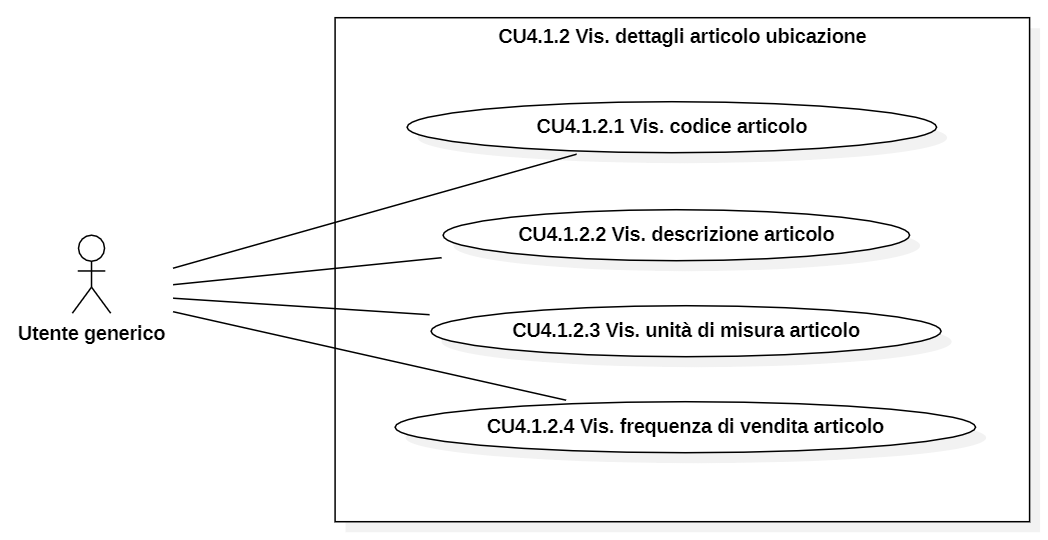
\includegraphics[width=1.2\columnwidth]{../images/usecase/form2/CU4_1_2} 
    }
    \caption{Casi d'uso - CU4.1.2 Vis. dettagli articolo ubicazione}
\end{figure}
%%%%%%%%%%%%%%%%%%%%%%%%%%%%%%%%%%%%%%%%%%%%%%%%%%%%%%
\begin{usecase}{4.1.2}{Vis. dettagli articolo ubicazione}
    \usecaseactors{Utente generico}
    \usecasepre{}
    \usecasedesc{L'utente visualizza i dettagli degli articoli presenti all'interno dell'ubicazione di magazzino}
    \usecasepost{I dettagli degli articoli presenti all'interno dell'ubicazione di magazzino sono visibili all'utente}
    \label{uc:scenario-principale}
\end{usecase}
%%%%%%%%%%%%%%%%%%%%%%%%%%%%%%%%%%%%%%%%%%%%%%%%%%%%%%
\begin{usecase}{4.1.2.1}{Vis. codice articolo}
    \usecaseactors{Utente generico}
    \usecasepre{Nessuna}
    \usecasedesc{L'utente visualizza il codice articolo dell'articolo contenuto nell'ubicazione di magazzino}
    \usecasepost{Il codice articolo dell'articolo presente nell'ubicazione di magazzino è visibile all'utente}
    \label{uc:scenario-principale}
\end{usecase}
%%%%%%%%%%%%%%%%%%%%%%%%%%%%%%%%%%%%%%%%%%%%%%%%%%%%%%
\begin{usecase}{4.1.2.2}{CU4.1.2.2 Vis. descrizione articolo}
    \usecaseactors{Utente generico}
    \usecasepre{Nessuna}
    \usecasedesc{L'utente visualizza la descrizione dell'articolo presente nell'ubicazione di magazzino}
    \usecasepost{La descrizione dell'articolo presente nell'ubicazione di magazzino è visibile all'utente}
    \label{uc:scenario-principale}
\end{usecase}
%%%%%%%%%%%%%%%%%%%%%%%%%%%%%%%%%%%%%%%%%%%%%%%%%%%%%%
\begin{usecase}{4.1.2.3}{CU4.1.2.3 Vis. unità di misura articolo}
    \usecaseactors{Utente generico}
    \usecasepre{Nessuna}
    \usecasedesc{L'utente visualizza l'unità di misura dell'articolo presente nell'ubicazione di magazzino}
    \usecasepost{L'unità di misura dell'articolo presente nell'ubicazione di magazzino è visibile all'utente}
    \label{uc:scenario-principale}
\end{usecase}
%%%%%%%%%%%%%%%%%%%%%%%%%%%%%%%%%%%%%%%%%%%%%%%%%%%%%%
\begin{usecase}{4.1.2.4}{CU4.1.2.4 Vis. frequenza di vendita articolo}
    \usecaseactors{Utente generico}
    \usecasepre{Nessuna}
    \usecasedesc{L'utente visualizza la frequenza di vendita dell'articolo presente nell'ubicazione di magazzino}
    \usecasepost{La frequenza di vendita dell'articolo presente nell'ubicazione di magazzino è visibile all'utente}
    \label{uc:scenario-principale}
\end{usecase}
%%%%%%%%%%%%%%%%%%%%%%%%%%%%%%%%%%%%%%%%%%%%%%%%%%%%%%
\begin{figure}[!h] 
    \centering 
    \makebox[\textwidth]{
    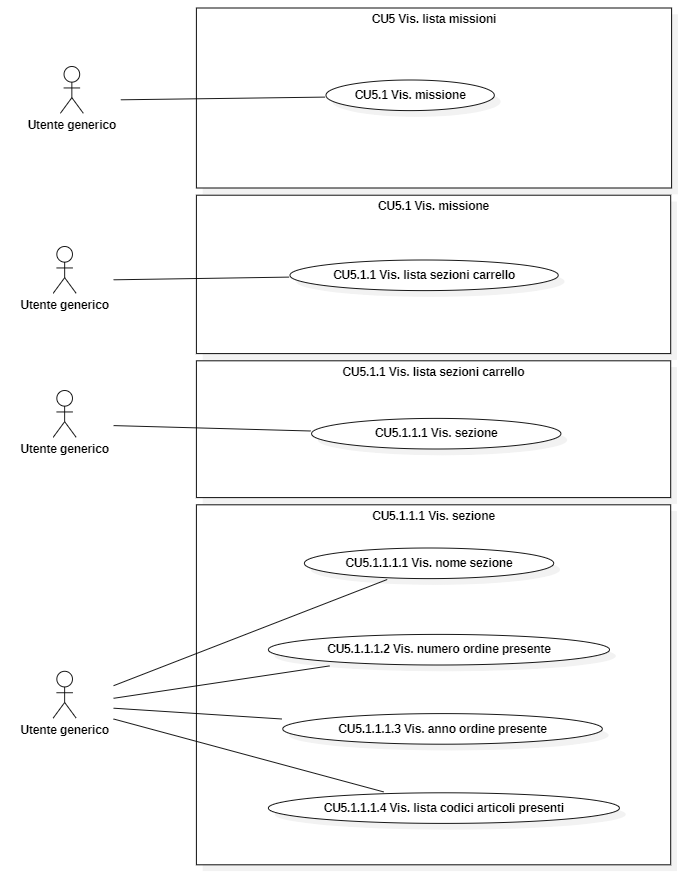
\includegraphics[width=1.2\columnwidth]{../images/usecase/form2/CU5_sottocasi} 
    }
    \caption{Casi d'uso - CU5 Vis. lista missioni}
\end{figure}
%%%%%%%%%%%%%%%%%%%%%%%%%%%%%%%%%%%%%%%%%%%%%%%%%%%%%%
\begin{usecase}{5}{Vis. lista missioni}
    \usecaseactors{Utente generico}
    \usecasepre{Nessuna}
    \usecasedesc{L'utente visualizza le missioni eseguite durante la simulazione di prelievo.}
    \usecasepost{Le missioni eseguite durante la simulazione di prelievo sono visibili all'utente}
    \label{uc:scenario-principale}
\end{usecase}
%%%%%%%%%%%%%%%%%%%%%%%%%%%%%%%%%%%%%%%%%%%%%%%%%%%%%%
\begin{usecase}{5.1}{Vis. missione}
    \usecaseactors{Utente generico}
    \usecasepre{Nessuna}
    \usecasedesc{L'utente visualizza la missione eseguita durante la simulazione di prelievo.}
    \usecasepost{La missione eseguita durante la simulazione di prelievo è visibile all'utente}
    \label{uc:scenario-principale}
\end{usecase}
%%%%%%%%%%%%%%%%%%%%%%%%%%%%%%%%%%%%%%%%%%%%%%%%%%%%%%
\begin{usecase}{5.1.1}{Vis. lista sezioni carrello}
    \usecaseactors{Utente generico}
    \usecasepre{Nessuna}
    \usecasedesc{L'utente visualizza le sezioni del carrello delle missioni. La lista delle sezioni del carrello rappresenta il carrello fisico che è il mezzo con cui vengono prelevati gli 
    articoli dalle ubicazioni di magazzino}
    \usecasepost{Le sezioni del carrello sono visibili all'utente}
    \label{uc:scenario-principale}
\end{usecase}
%%%%%%%%%%%%%%%%%%%%%%%%%%%%%%%%%%%%%%%%%%%%%%%%%%%%%%
\begin{usecase}{5.1.1.1}{Vis. sezione}
    \usecaseactors{Utente generico}
    \usecasepre{Nessuna}
    \usecasedesc{L'utente visualizza una sezione del carrello. Una sezione del carrello corrisponde ad una zona di carrello in cui è possibile collocare gli articoli di un ordine}
    \usecasepost{La sezione del carrello è visibile all'utente}
    \label{uc:scenario-principale}
\end{usecase}
%%%%%%%%%%%%%%%%%%%%%%%%%%%%%%%%%%%%%%%%%%%%%%%%%%%%%%
\begin{usecase}{5.1.1.1.1}{Vis. nome sezione}
    \usecaseactors{Utente generico}
    \usecasepre{Nessuna}
    \usecasedesc{L'utente visualizza il nome della sezione del carrello. Il nome segue una numerazione incrementale che corrisponde alla posizione in cui si trova la 
    sezione rispetto alla sezione di coda del carrello. La sezione di coda ha numerazione pari a 1 ed è il numero di sezione più basso}
    \usecasepost{Il nome della sezione del carrello è visibile all'utente}
    \label{uc:scenario-principale}
\end{usecase}
%%%%%%%%%%%%%%%%%%%%%%%%%%%%%%%%%%%%%%%%%%%%%%%%%%%%%%
\begin{usecase}{5.1.1.1.2}{Vis. numero ordine presente}
    \usecaseactors{Utente generico}
    \usecasepre{Nessuna}
    \usecasedesc{L'utente visualizza il numero dell'ordine presente nella sezione del carrello. All'interno di una sezione può essere presente un ordine alla volta}
    \usecasepost{Il numero dell'ordine presente nella sezione del carrello è visibile all'utente}
    \label{uc:scenario-principale}
\end{usecase}
%%%%%%%%%%%%%%%%%%%%%%%%%%%%%%%%%%%%%%%%%%%%%%%%%%%%%%
\begin{usecase}{5.1.1.1.3}{Vis. anno ordine presente}
    \usecaseactors{Utente generico}
    \usecasepre{Nessuna}
    \usecasedesc{L'utente visualizza l'anno dell'ordine presente nella sezione del carrello. L'anno dell'ordine indica l'anno in cui l'ordine è stato emesso}
    \usecasepost{L'anno dell'ordine presente nella sezione del carrello è visibile all'utente}
    \label{uc:scenario-principale}
\end{usecase}
%%%%%%%%%%%%%%%%%%%%%%%%%%%%%%%%%%%%%%%%%%%%%%%%%%%%%%
\begin{usecase}{5.1.1.1.4}{Vis. lista codici articoli presenti}
    \usecaseactors{Utente generico}
    \usecasepre{Nessuna}
    \usecasedesc{L'utente visualizza la lista dei codici articoli presenti nella sezione del carrello. Il codice articolo è un identificatore univoco per ogni articolo}
    \usecasepost{La lista dei codici articoli presenti nella sezione del carrello è visibile all'utente}
    \label{uc:scenario-principale}
\end{usecase}
%%%%%%%%%%%%%%%%%%%%%%%%%%%%%%%%%%%%%%%%%%%%%%%%%%%%%%
\begin{figure}[!h] 
    \centering 
    \makebox[\textwidth]{
    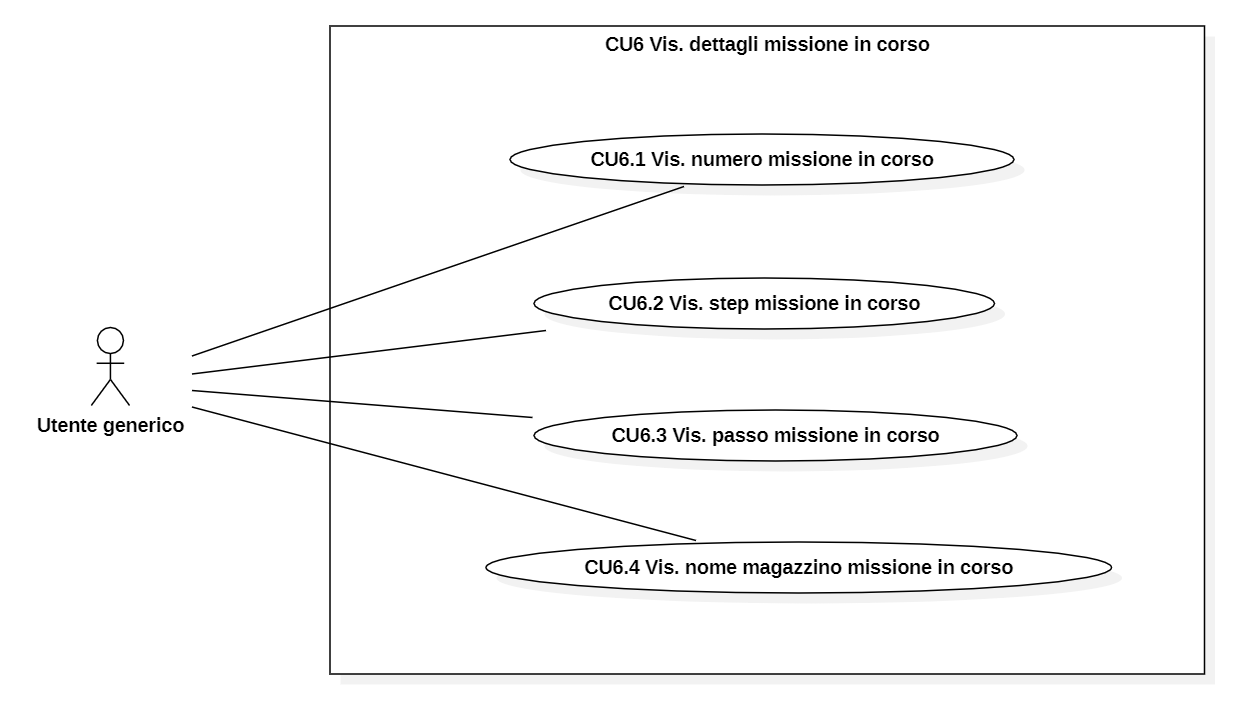
\includegraphics[width=1.2\columnwidth]{../images/usecase/form2/CU6} 
    }
    \caption{Casi d'uso - CU6 Vis. dettagli missione in corso}
\end{figure}
%%%%%%%%%%%%%%%%%%%%%%%%%%%%%%%%%%%%%%%%%%%%%%%%%%%%%%
\begin{usecase}{6}{Vis. dettagli missione in corso}
    \usecaseactors{Utente generico}
    \usecasepre{Nessuna}
    \usecasedesc{L'utente visualizza i dettagli della missione in corso}
    \usecasepost{I dettagli della missione in corso sono visibili all'utente}
    \label{uc:scenario-principale}
\end{usecase}
%%%%%%%%%%%%%%%%%%%%%%%%%%%%%%%%%%%%%%%%%%%%%%%%%%%%%%
\begin{usecase}{6.1}{Vis. numero missione in corso}
    \usecaseactors{Utente generico}
    \usecasepre{Nessuna}
    \usecasedesc{L'utente visualizza il numero della missione in corso}
    \usecasepost{Il numero della missione in corso è visibile all'utente}
    \label{uc:scenario-principale}
\end{usecase}
%%%%%%%%%%%%%%%%%%%%%%%%%%%%%%%%%%%%%%%%%%%%%%%%%%%%%%
\begin{usecase}{6.2}{Vis. step missione in corso}
    \usecaseactors{Utente generico}
    \usecasepre{Nessuna}
    \usecasedesc{L'utente visualizza lo step della missione in corso. Lo step corrisponde al numero di fermate attuale effettuate dal carrello}
    \usecasepost{Lo step della missione in corso è visibile all'utente}
    \label{uc:scenario-principale}
\end{usecase}
%%%%%%%%%%%%%%%%%%%%%%%%%%%%%%%%%%%%%%%%%%%%%%%%%%%%%%
\begin{usecase}{6.3}{Vis. passo missione in corso}
    \usecaseactors{Utente generico}
    \usecasepre{Nessuna}
    \usecasedesc{L'utente visualizza il passo della missione in corso. Il passo corrisponde al numero di articoli associati che vengono messi nelle ubicazioni contigue ad ogni articolo.
    Il passo di associazione è un fattore che caratterizza la missione in quanto l'obiettivo di una simulazione di prelievo è valutare quale sia il passo missione migliore per completare gli ordini}
    \usecasepost{Il passo della missione in corso è visibile all'utente}
    \label{uc:scenario-principale}
\end{usecase}
%%%%%%%%%%%%%%%%%%%%%%%%%%%%%%%%%%%%%%%%%%%%%%%%%%%%%%
\begin{usecase}{6.4}{Vis. nome magazzino missione in corso}
    \usecaseactors{Utente generico}
    \usecasepre{Nessuna}
    \usecasedesc{L'utente visualizza il nome del magazzino nel quale avviene la simulazione di prelievo e quindi la missione in corso}
    \usecasepost{Il nome del magazzino della missione in corso è visibile all'utente}
    \label{uc:scenario-principale}
\end{usecase}
%%%%%%%%%%%%%%%%%%%%%%%%%%%%%%%%%%%%%%%%%%%%%%%%%%%%%%
\begin{figure}[!h] 
    \centering 
    \makebox[\textwidth]{
    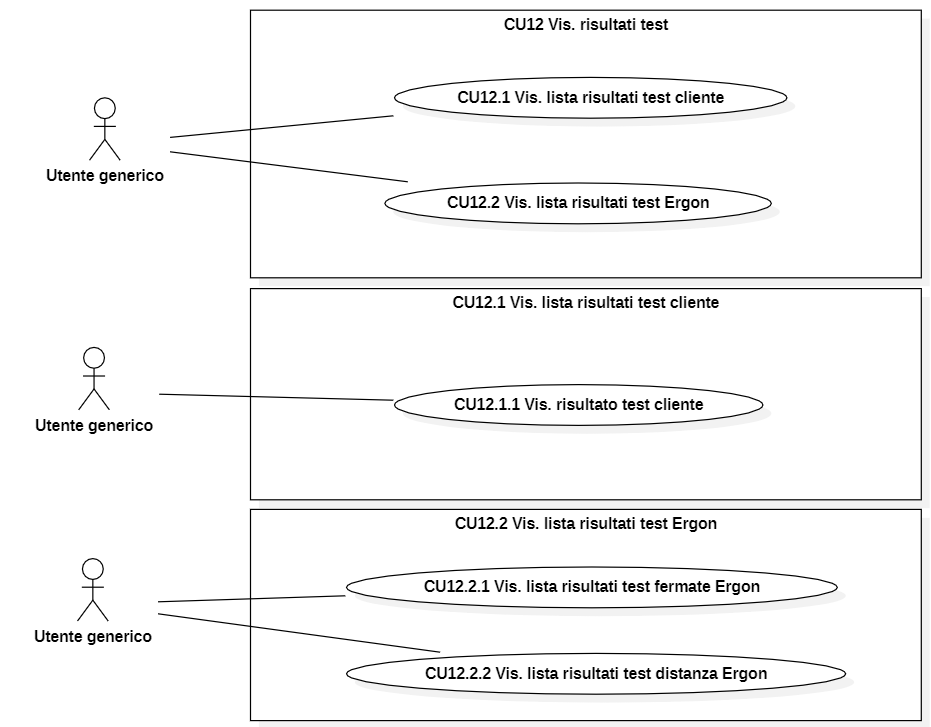
\includegraphics[width=1.2\columnwidth]{../images/usecase/form3/CU12_sottocasi1} 
    }
    \caption{Casi d'uso - CU12 Vis. risultati test}
\end{figure}
%%%%%%%%%%%%%%%%%%%%%%%%%%%%%%%%%%%%%%%%%%%%%%%%%%%%%%
\begin{usecase}{12}{Vis. risultati test}
    \usecaseactors{Utente generico}
    \usecasepre{Nessuna}
    \usecasedesc{L'utente visualizza i risultati dei test della missione di prelievo. La visualizzazione dei risultati dei test permette di capire quali sono i parametri di test che portano 
    ad una migliore configurazione del magazzino}
    \usecasepost{I risultati dei test della missione di prelievo sono visibili all'utente}
    \label{uc:scenario-principale}
\end{usecase}
%%%%%%%%%%%%%%%%%%%%%%%%%%%%%%%%%%%%%%%%%%%%%%%%%%%%%% CLIENTE
\begin{usecase}{12.1}{Vis. lista risultati test cliente}
    \usecaseactors{Utente generico}
    \usecasepre{Nessuna}
    \usecasedesc{L'utente visualizza i risultati dei test effettuati sul magazzino del cliente. Il magazzino del cliente non prevede nessuna configurazione con passi associazioni prodotti e 
    rispecchia l'attuale configurazione del magazzino del cliente}
    \usecasepost{I risultati dei test effettuati sul magazzino del cliente sono visibili all'utente}
    \label{uc:scenario-principale}
\end{usecase}
%%%%%%%%%%%%%%%%%%%%%%%%%%%%%%%%%%%%%%%%%%%%%%%%%%%%%%
\begin{usecase}{12.1.1}{Vis. risultato test cliente}
    \usecaseactors{Utente generico}
    \usecasepre{Nessuna}
    \usecasedesc{L'utente visualizza il risultato del test effettuato sul magazzino del cliente}
    \usecasepost{Il risultato del test effettuato sul magazzino cliente è visibile all'utente}
    \label{uc:scenario-principale}
\end{usecase}





%%%%%%%%%%%%%%%%%%%%%%%%%%%%%%%%%%%%%%%%%%%%%%%%%%%%%%
\begin{usecase}{12.1.1.1}{Vis. nome cliente}
    \usecaseactors{Utente generico}
    \usecasepre{Nessuna}
    \usecasedesc{L'utente visualizza il nome del cliente proprietario del magazzino di test}
    \usecasepost{Il nome del cliente è visibile all'utente}
    \label{uc:scenario-principale}
\end{usecase}
%%%%%%%%%%%%%%%%%%%%%%%%%%%%%%%%%%%%%%%%%%%%%%%%%%%%%%
\begin{usecase}{12.1.1.2}{Vis. codice deposito}
    \usecaseactors{Utente generico}
    \usecasepre{Nessuna}
    \usecasedesc{L'utente visualizza il codice del deposito sul quale viene effettuato il test}
    \usecasepost{Il codice del deposito del cliente è visibile all'utente}
    \label{uc:scenario-principale}
\end{usecase}
%%%%%%%%%%%%%%%%%%%%%%%%%%%%%%%%%%%%%%%%%%%%%%%%%%%%%%
\begin{usecase}{12.1.1.3}{Vis. tipo test}
    \usecaseactors{Utente generico}
    \usecasepre{Nessuna}
    \usecasedesc{L'utente visualizza il tipo di test. Il tipo di test ne caratterizza la modalità e il risultato finale. Sono previsti test sulle fermate e test sulle distanze percorse}
    \usecasepost{Il tipo di test effettuato è visibile all'utente}
    \label{uc:scenario-principale}
\end{usecase}
%%%%%%%%%%%%%%%%%%%%%%%%%%%%%%%%%%%%%%%%%%%%%%%%%%%%%%
\begin{usecase}{12.1.1.4}{Vis. dimensione carrello}
    \usecaseactors{Utente generico}
    \usecasepre{Nessuna}
    \usecasedesc{L'utente visualizza la dimensione del carrello. La dimensione del carrello corrisponde al numero di sezioni che compongono il carrello}
    \usecasepost{La dimensione del carrello è visibile all'utente}
    \label{uc:scenario-principale}
\end{usecase}
%%%%%%%%%%%%%%%%%%%%%%%%%%%%%%%%%%%%%%%%%%%%%%%%%%%%%%
\begin{usecase}{12.1.1.5}{Vis. descrizione}
    \usecaseactors{Utente generico}
    \usecasepre{Nessuna}
    \usecasedesc{L'utente visualizza la descrizione del test effettuato sul magazzino del cliente. La descrizione è una breve frase che riassume le caratteristiche principali del test}
    \usecasepost{La descrizione del test è visibile all'utente}
    \label{uc:scenario-principale}
\end{usecase}
%%%%%%%%%%%%%%%%%%%%%%%%%%%%%%%%%%%%%%%%%%%%%%%%%%%%%%
\begin{usecase}{12.1.1.6}{Vis. risultato}
    \usecaseactors{Utente generico}
    \usecasepre{Nessuna}
    \usecasedesc{L'utente visualizza il risultato del test effettuato sul magazzino del cliente. Il risultato varia a seconda del tipo di test e per questo è seguito dall'unità di misura opportuna.}
    \usecasepost{Il risultato del test effettuato sul magazzino cliente è visibile all'utente}
    \label{uc:scenario-principale}
\end{usecase}










%%%%%%%%%%%%%%%%%%%%%%%%%%%%%%%%%%%%%%%%%%%%%%%%%%%%%% ERGON
\begin{usecase}{12.2}{Vis. lista risultati test Ergon}
    \usecaseactors{Utente generico}
    \usecasepre{Nessuna}
    \usecasedesc{L'utente visualizza i risultati dei test effettuati sul magazzino Ergon. Il magazzino Ergon prevede una configurazione con passi associazioni prodotti. Ogni 
    test su ciascun passo associazione produce un risultato che viene visualizzato}
    \usecasepost{I risultati dei test effettuati sul magazzino Ergon sono visibili all'utente}
    \label{uc:scenario-principale}
\end{usecase}
%%%%%%%%%%%%%%%%%%%%%%%%%%%%%%%%%%%%%%%%%%%%%%%%%%%%%%
\begin{usecase}{12.2.1}{Vis. lista risultati test fermate Ergon}
    \usecaseactors{Utente generico}
    \usecasepre{Nessuna}
    \usecasedesc{L'utente visualizza i risultati dei test sulle fermate effettuati sul magazzino Ergon. La funzionalità prevede la visualizzazione di un enfasi sugli elementi della 
    lista che corrispondono ai migliori risultati e ai peggiori risultati. Il miglior risultato è quello che ha prodotto il minor numero di fermate del carrello durante la 
    simulazione di prelievo.  Il peggior risultato è quello che ha prodotto il maggior numero di fermate del carrello durante la 
    simulazione di prelievo. In caso di parità sarà enfatizzato il risultato che ha come passo associazione il passo del risultato dei test sulle distanze che ha prodotto la minor distanza
    percorsa a parità di passo associazine. Nel caso in cui il miglior risultato corrisponda anche al peggior risultato sarà applicata un'enfasi specifica}
    \textbf{\\Postcondizioni:}
\begin{itemize}
    \item I risultati dei test sulle fermate effettuati sul magazzino Ergon sono visibili all'utente;
    \item L'elemento che corrisponde al risultato migliore è enfatizzato;
    \item L'elemento che corrisponde al risultato peggiore è enfatizzato;
\end{itemize}
    \label{uc:scenario-principale}
\end{usecase}
%%%%%%%%%%%%%%%%%%%%%%%%%%%%%%%%%%%%%%%%%%%%%%%%%%%%%%
\begin{usecase}{12.2.2}{Vis. lista risultati test distanza Ergon}
    \usecaseactors{Utente generico}
    \usecasepre{Nessuna}
    \usecasedesc{L'utente visualizza i risultati dei test sulle distanze effettuati sul magazzino Ergon. La funzionalità prevede la visualizzazione di un enfasi sugli elementi della 
    lista che corrispondono ai migliori risultati e ai peggiori risultati. Il miglior risultato è quello che ha prodotto una distanza percorsa minore del carrello durante la 
    simulazione di prelievo.  Il peggior risultato è quello che ha prodotto una distanza percorsa maggiore del carrello durante la 
    simulazione di prelievo. Nel caso in cui il miglior risultato corrisponda anche al peggior risultato sarà applicata un'enfasi specifica}
    \textbf{\\Postcondizioni:}
\begin{itemize}
    \item I risultati dei test sulle distanza effettuati sul magazzino Ergon sono visibili all'utente;
    \item L'elemento che corrisponde al risultato migliore è enfatizzato;
    \item L'elemento che corrisponde al risultato peggiore è enfatizzato;
\end{itemize}
    \label{uc:scenario-principale}
\end{usecase}
%%%%%%%%%%%%%%%%%%%%%%%%%%%%%%%%%%%%%%%%%%%%%%%%%%%%%%
\begin{usecase}{12.2.1.1}{Vis. risultato test fermate Ergon}
    \usecaseactors{Utente generico}
    \usecasepre{Nessuna}
    \usecasedesc{L'utente visualizza il risultato del test sulle fermate effettuato sul magazzino Ergon}
    \usecasepost{Il risultato del test sulle fermate effettuati sul magazzino Ergon è visibile all'utente}
    \label{uc:scenario-principale}
\end{usecase}
%%%%%%%%%%%%%%%%%%%%%%%%%%%%%%%%%%%%%%%%%%%%%%%%%%%%%%
\begin{usecase}{12.2.2.1}{Vis. risultato test distanza Ergon}
    \usecaseactors{Utente generico}
    \usecasepre{Nessuna}
    \usecasedesc{L'utente visualizza il risultato del test sulla distanza effettuato sul magazzino Ergon}
    \usecasepost{Il risultato del test sulla distanza effettuato sul magazzino Ergon è visibile all'utente}
    \label{uc:scenario-principale}
\end{usecase}
%%%%%%%%%%%%%%%%%%%

%%%%%%%%%%%%%%%%%%%%%%%%%%%%%%%%%%%%%%%%%%%%%%%%%%%%%%
\begin{usecase}{12.2.1.1.1}{Vis. tipo}
    \usecaseactors{Utente generico}
    \usecasepre{Nessuna}
    \usecasedesc{L'utente visualizza il tipo di test effettuato}
    \usecasepost{Il tipo del test effettuato è visibile all'utente}
    \label{uc:scenario-principale}
\end{usecase}
%%%%%%%%%%%%%%%%%%%%%%%%%%%%%%%%%%%%%%%%%%%%%%%%%%%%%%
\begin{usecase}{12.2.1.1.2}{Vis. descrizione}
    \usecaseactors{Utente generico}
    \usecasepre{Nessuna}
    \usecasedesc{L'utente visualizza la descrizione del test effettuato}
    \usecasepost{La descrizione del test è visibile all'utente}
    \label{uc:scenario-principale}
\end{usecase}
%%%%%%%%%%%%%%%%%%%%%%%%%%%%%%%%%%%%%%%%%%%%%%%%%%%%%%
\begin{usecase}{12.2.1.1.3}{Vis. dimensione carrello}
    \usecaseactors{Utente generico}
    \usecasepre{Nessuna}
    \usecasedesc{L'utente visualizza la dimensione del carrello con il quale è stato effettuato il test. La dimensione del carrello corrisponde al numero di ordini che il carrello è in grado di 
    completare}
    \usecasepost{La dimensione del carrello è visibile all'utente}
    \label{uc:scenario-principale}
\end{usecase}
%%%%%%%%%%%%%%%%%%%%%%%%%%%%%%%%%%%%%%%%%%%%%%%%%%%%%%
\begin{usecase}{12.2.1.1.4}{Vis. passo associazioni}
    \usecaseactors{Utente generico}
    \usecasepre{Nessuna}
    \usecasedesc{L'utente visualizza il passo associazioni con cui è stato effettuato il test}
    \usecasepost{Il passo associazioni con cui è stato effettuato il test è visibile all'utente}
    \label{uc:scenario-principale}
\end{usecase}
%%%%%%%%%%%%%%%%%%%%%%%%%%%%%%%%%%%%%%%%%%%%%%%%%%%%%%
\begin{usecase}{12.2.1.1.5}{Vis. numero fermate}
    \usecaseactors{Utente generico}
    \usecasepre{Nessuna}
    \usecasedesc{L'utente visualizza il numero di fermate impiegate per completare la simulazione di prelievo}
    \usecasepost{Il numero di fermate impiegate per completare la simulazione di prelievo è visibile all'utente}
    \label{uc:scenario-principale}
\end{usecase}





%%%%%%%%%%%%%%%%%%%%%%%%%%%%%%%%%%%%%%%%%%%%%%%%%%%%%%
\begin{usecase}{12.2.2.1.1}{Vis. tipo}
    \usecaseactors{Utente generico}
    \usecasepre{Nessuna}
    \usecasedesc{L'utente visualizza il tipo di test effettuato}
    \usecasepost{Il tipo del test effettuato è visibile all'utente}
    \label{uc:scenario-principale}
\end{usecase}
%%%%%%%%%%%%%%%%%%%%%%%%%%%%%%%%%%%%%%%%%%%%%%%%%%%%%%
\begin{usecase}{12.2.2.1.2}{Vis. descrizione}
    \usecaseactors{Utente generico}
    \usecasepre{Nessuna}
    \usecasedesc{L'utente visualizza la descrizione del test effettuato}
    \usecasepost{La descrizione del test è visibile all'utente}
    \label{uc:scenario-principale}
\end{usecase}
%%%%%%%%%%%%%%%%%%%%%%%%%%%%%%%%%%%%%%%%%%%%%%%%%%%%%%
\begin{usecase}{12.2.2.1.3}{Vis. dimensione carrello}
    \usecaseactors{Utente generico}
    \usecasepre{Nessuna}
    \usecasedesc{L'utente visualizza la dimensione del carrello con il quale è stato effettuato il test. La dimensione del carrello corrisponde al numero di ordini che il carrello è in grado di 
    completare}
    \usecasepost{La dimensione del carrello è visibile all'utente}
    \label{uc:scenario-principale}
\end{usecase}
%%%%%%%%%%%%%%%%%%%%%%%%%%%%%%%%%%%%%%%%%%%%%%%%%%%%%%
\begin{usecase}{12.2.2.1.4}{Vis. passo associazioni}
    \usecaseactors{Utente generico}
    \usecasepre{Nessuna}
    \usecasedesc{L'utente visualizza il passo associazioni con cui è stato effettuato il test}
    \usecasepost{Il passo associazioni con cui è stato effettuato il test è visibile all'utente}
    \label{uc:scenario-principale}
\end{usecase}
%%%%%%%%%%%%%%%%%%%%%%%%%%%%%%%%%%%%%%%%%%%%%%%%%%%%%%
\begin{usecase}{12.2.2.1.5}{Vis. ubicazioni percorse}
    \usecaseactors{Utente generico}
    \usecasepre{Nessuna}
    \usecasedesc{L'utente visualizza il numero di ubicazioni percorse dal carrello per completare la simulazione di prelievo}
    \usecasepost{Il numero di ubicazioni percorse dal carrello per completare la simulazione di prelievo è visibile all'utente}
    \label{uc:scenario-principale}
\end{usecase}









%%%%%%%%%%%%%%%%%%%%%%%%%%%%%%%%%%%%%%%%%%%%%%%%%%%%%%
\begin{figure}[!h] 
    \centering 
    \makebox[\textwidth]{
    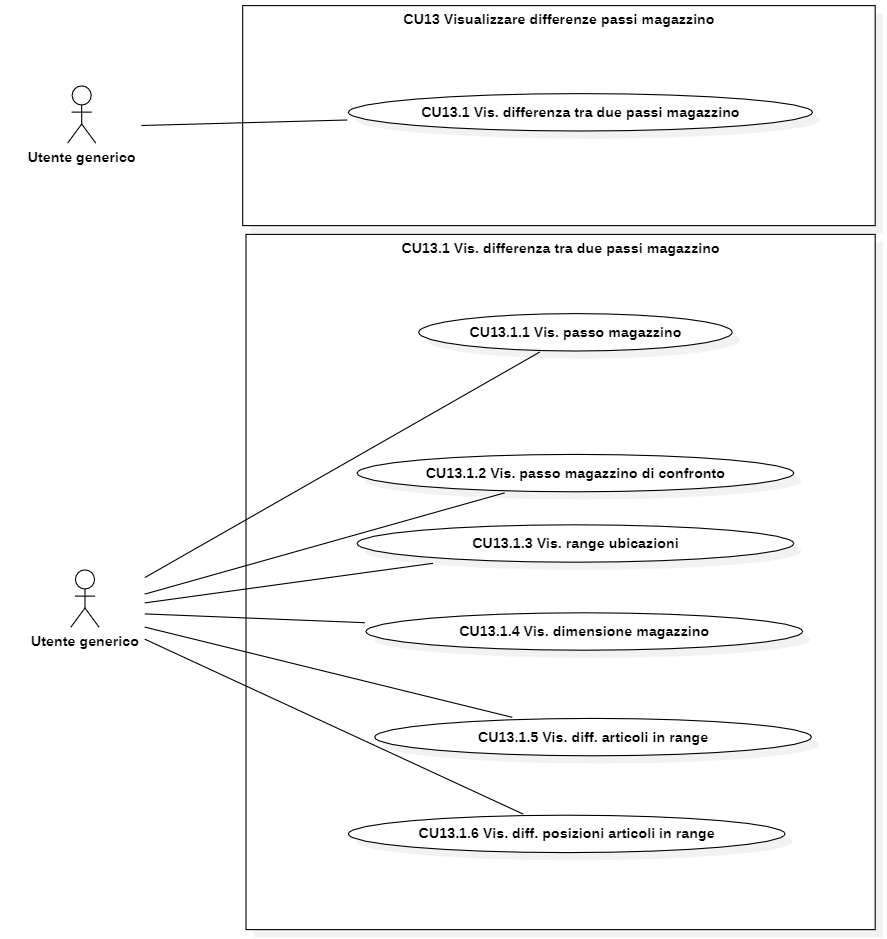
\includegraphics[width=1.2\columnwidth]{../images/usecase/form4/CU13_sottocasi} 
    }
    \caption{Casi d'uso - CU13 Visualizzare differenze passi magazzino}
\end{figure}
%%%%%%%%%%%%%%%%%%%%%%%%%%%%%%%%%%%%%%%%%%%%%%%%%%%%%%
\begin{usecase}{13}{Visualizzare differenze passi magazzino}
    \usecaseactors{Utente generico}
    \usecasepre{Nessuna}
    \usecasedesc{L'utente visualizza le differenze tra i passi di magazzino in un range scelto dall'utente}
    \usecasepost{Le differenze tra i passi di magazzino sono visibili all'utente}
    \label{uc:scenario-principale}
\end{usecase}
%%%%%%%%%%%%%%%%%%%%%%%%%%%%%%%%%%%%%%%%%%%%%%%%%%%%%%
\begin{usecase}{13.1}{Vis. differenza tra due passi magazzino}
    \usecaseactors{Utente generico}
    \usecasepre{Nessuna}
    \usecasedesc{L'utente visualizza le differenze tra due passi di magazzino}
    \usecasepost{Le differenze tra due passi di magazzino sono visibili all'utente}
    \label{uc:scenario-principale}
\end{usecase}
%%%%%%%%%%%%%%%%%%%%%%%%%%%%%%%%%%%%%%%%%%%%%%%%%%%%%%
\begin{usecase}{13.1.1}{Vis. passo magazzino}
    \usecaseactors{Utente generico}
    \usecasepre{Nessuna}
    \usecasedesc{L'utente visualizza il passo del magazzino che si vuole confrontare con un passo di confronto}
    \usecasepost{Il passo di magazzino che si vuole confrontare con un passo di confronto è visibile all'utente}
    \label{uc:scenario-principale}
\end{usecase}
%%%%%%%%%%%%%%%%%%%%%%%%%%%%%%%%%%%%%%%%%%%%%%%%%%%%%%
\begin{usecase}{13.1.2}{Vis. passo magazzino di confronto}
    \usecaseactors{Utente generico}
    \usecasepre{Nessuna}
    \usecasedesc{L'utente visualizza il passo del magazzino di confronto}
    \usecasepost{Il passo di magazzino di confronto è visibile all'utente}
    \label{uc:scenario-principale}
\end{usecase}
%%%%%%%%%%%%%%%%%%%%%%%%%%%%%%%%%%%%%%%%%%%%%%%%%%%%%%
\begin{usecase}{13.1.3}{Vis. range ubicazioni}
    \usecaseactors{Utente generico}
    \usecasepre{Nessuna}
    \usecasedesc{L'utente visualizza il range entro il quale vengono confrontate le ubicazioni di magazzino tra le diverse configurazioni determinate dal passo associazione}
    \usecasepost{Il range entro il quale vengono confrontate le ubicazioni di magazzi è visibile all'utente}
    \label{uc:scenario-principale}
\end{usecase}
%%%%%%%%%%%%%%%%%%%%%%%%%%%%%%%%%%%%%%%%%%%%%%%%%%%%%%
\begin{usecase}{13.1.4}{Vis. dimensione magazzino}
    \usecaseactors{Utente generico}
    \usecasepre{Nessuna}
    \usecasedesc{L'utente visualizza la dimensione del magazzino. La dimensione del magazzino è determinata dagli articoli che contiene in quanto un'ubicazione contiene un solo codice articolo.
    Si suppone che tutti gli articoli disponibili siano contenuti all'interno del magazzino}
    \usecasepost{La dimensione del magazzino è visibile all'utente}
    \label{uc:scenario-principale}
\end{usecase}
%%%%%%%%%%%%%%%%%%%%%%%%%%%%%%%%%%%%%%%%%%%%%%%%%%%%%%
\begin{usecase}{13.1.5}{Vis. diff. articoli in range}
    \usecaseactors{Utente generico}
    \usecasepre{Nessuna}
    \usecasedesc{L'utente visualizza il numero (conteggio incrementale) dei codici articoli che non sono presenti nella prima configurazione rispetto alla configurazione di confronto entro il 
    range fissato dall'utente}
    \usecasepost{Il numero di differenze di codici articoli tra la configurazione di magazzino e la configurazione di confronto è visibile all'utente}
    \label{uc:scenario-principale}
\end{usecase}
%%%%%%%%%%%%%%%%%%%%%%%%%%%%%%%%%%%%%%%%%%%%%%%%%%%%%%
\begin{usecase}{13.1.6}{Vis. diff. posizioni articoli in range}
    \usecaseactors{Utente generico}
    \usecasepre{Nessuna}
    \usecasedesc{L'utente visualizza il numero (conteggio incrementale) dei codici articoli che non si trovano più nella stessa ubicazione nella configurazione 
    di confronto rispetto alla configurazione di magazzino entro il range fissato dall'utente}
    \usecasepost{Il numero dei codici articoli che non si trovano più nella stessa ubicazione sono visibili all'utente}
    \label{uc:scenario-principale}
\end{usecase}




\section{Tracciamento dei requisiti}

Da un'attenta analisi dei requisiti e degli use case effettuata sul progetto è stata stilata la tabella che traccia i requisiti in rapporto agli use case.\\
Sono stati individuati diversi tipi di requisiti e si è quindi fatto utilizzo di un codice identificativo per distinguerli.\\
Il codice dei requisiti è così strutturato R(F/Q/V)(N/D/O) dove:
\begin{enumerate}
	\item[R =] requisito
    \item[F =] funzionale
    \item[Q =] qualitativo
    \item[V =] di vincolo
    \item[N =] obbligatorio (necessario)
    \item[D =] desiderabile
    \item[Z =] opzionale
\end{enumerate}
Nelle tabelle \ref{tab:requisiti-funzionali}, \ref{tab:requisiti-qualitativi} e \ref{tab:requisiti-vincolo} sono riassunti i requisiti e il loro tracciamento con gli use case delineati in fase di analisi.

\newpage

\begin{table}
\caption{Tabella del tracciamento dei requisti funzionali}
\label{tab:requisiti-funzionali}
\begin{tabularx}{\textwidth}{lXl}
\hline\hline
\textbf{Requisito} & \textbf{Descrizione} & \textbf{Use Case}\\
\hline
RFN-1     & L'interfaccia utente permette di visualizzare gli articoli in forma tabellare & UC1 \\
RFN-2     & L'interfaccia utente evidenzia l'articolo di cui si sta visualizzando gli articoli associati & UC2 \\
RFN-3     & L'interfaccia utente permette di selezionare un articolo di cui si vogliono visualizzare gli articoli associati & UC2 \\ 
RFN-4     & L'interfaccia utente deve aggiornare i dati visualizzati al termine dell'operazione di aggiornamento dei dati a database & UC3 \\ 
RFN-5     & L'interfaccia utente prevede la visualizzazione di un messaggio informativo che informi l'utente di attendere il termine dell'aggiornamento dei dati prima di compiere qualsiasi altra
interazione con il sistema & UC3 \\ 
RFN-6     & L'interfaccia utente deve permettere di visualizzare in ordine crescente per posizione le ubicazioni di magazzino e non deve permettere l'alterazione di questo ordine & UC4 \\ 
RFN-7     & L'interfaccia utente deve permettere di visualizzare in ordine crescente per esecuzione le missioni di prelievo eseguite e non deve permetterne l'alterazione di questo ordine & UC5 \\ 
RFN-8     & Il sistema deve tenere traccia della missione in corso e delle caratteristiche che la identificano & UC6 \\ 
RFN-9     & L'interfaccia utente permette l'interruzione della missione di prelievo in corso & UC7 UC8\\ 
RFN-10    & L'interfaccia utente deve ripristinare il suo stato iniziale con una configurazione di magazzino che rispetti il passo selezionato & UC7 \\ 
RFN-11    & L'interfaccia utente deve ripristinare il suo stato iniziale con una configurazione di magazzino che rispetti il magazzino selezionato & UC8 \\ 
RFN-12    & Il sistema deve permettere l'esecuzione e la visualizzazione di una simulazione di prelievo per una sola configurazione di magazzino alla volta & UC9 UC10 \\ 
RFN-13    & Il sistema deve permettere il reset automatico dello step della missione in corso al suo termine & UC11 \\ 
RFN-14    & Il sistema deve avvisare l'utente del termine di una missione di prelievo & UC11 \\ 
RFN-15    & Il sistema deve avvisare l'utente del termine di tutte le missioni di prelievo & UC11 \\ 
RFN-16    & Il sistema deve disabilitare la funzionalità di avanzamento step missione in corso al termine di tutte le missioni di prelievo & UC11 \\ 
RFN-17    & Il sistema deve poter eseguire tutti i test previsti per poter fornire all'utente i loro risultati in forma tabellare  & UC12 \\ 
RFN-17    & L'interfaccia utente deve rendere distinguibili i risultati dei test effettuati sul magazzino cliente dai test effettuati sul magazzino Ergon  & UC12 \\ 
RFN-18    & L'interfaccia utente deve permettere all'utente un facile confronto tra i risultati dei test visualizzati  & UC12 \\ 
RFN-18    & Il sistema deve   & UC12 \\ 
RFN-19    & L'interfaccia utente deve permettere all'utente un facile confronto tra i passi di magazzino visualizzati & UC13 \\ 
RFN-20    & L'interfaccia utente deve aggiornare i dati sulle differenze passi visualizzati alla modifica del range & UC14 \\ 

\hline
\end{tabularx}
\end{table}

\begin{table}
\caption{Tabella del tracciamento dei requisiti qualitativi}
\label{tab:requisiti-qualitativi}
\begin{tabularx}{\textwidth}{lXl}
\hline\hline
\textbf{Requisito} & \textbf{Descrizione} & \textbf{Use Case}\\
\hline
RQD-1    & Le prestazioni del simulatore hardware deve garantire la giusta esecuzione dei test e non la generazione di falsi negativi & - \\
\hline
\end{tabularx}
\end{table}

\begin{table}
    \caption{Tabella del tracciamento dei requisiti di vincolo}
\label{tab:requisiti-vincolo}
\begin{tabularx}{\textwidth}{lXl}
\hline\hline
\textbf{Requisito} & \textbf{Descrizione} & \textbf{Use Case}\\
\hline
RVN-1     & Il sistema deve essere in grado di stabilire una connessione con il database Informix del cliente & UC3 \\ 
RVN-2     & Il sistema deve avere i permessi di lettura e scrittura sui dati contenuti nel database Informix del cliente & UC3 \\ 

\hline
\end{tabularx}
\end{table}
